\chapter{Обгрунтування методології проектування та постановка задачі}
\label{chap:second}

\section{Обгрунтування методології проектування та функціональна модель задачі}

Методологією проектування обрана модель waterfall \cite{waterfall}, тому що предметна область не відрізняється високою динамікою на ринку а тому і в плані вимог. Обрана модель забезпечує оптимальний процесс створення системи.

Стандартом за яким проводиться опис ІС було обрано UML, середовище - UML Designer 9.0

Функціональна модель системи наведено нище:

\begin{center}

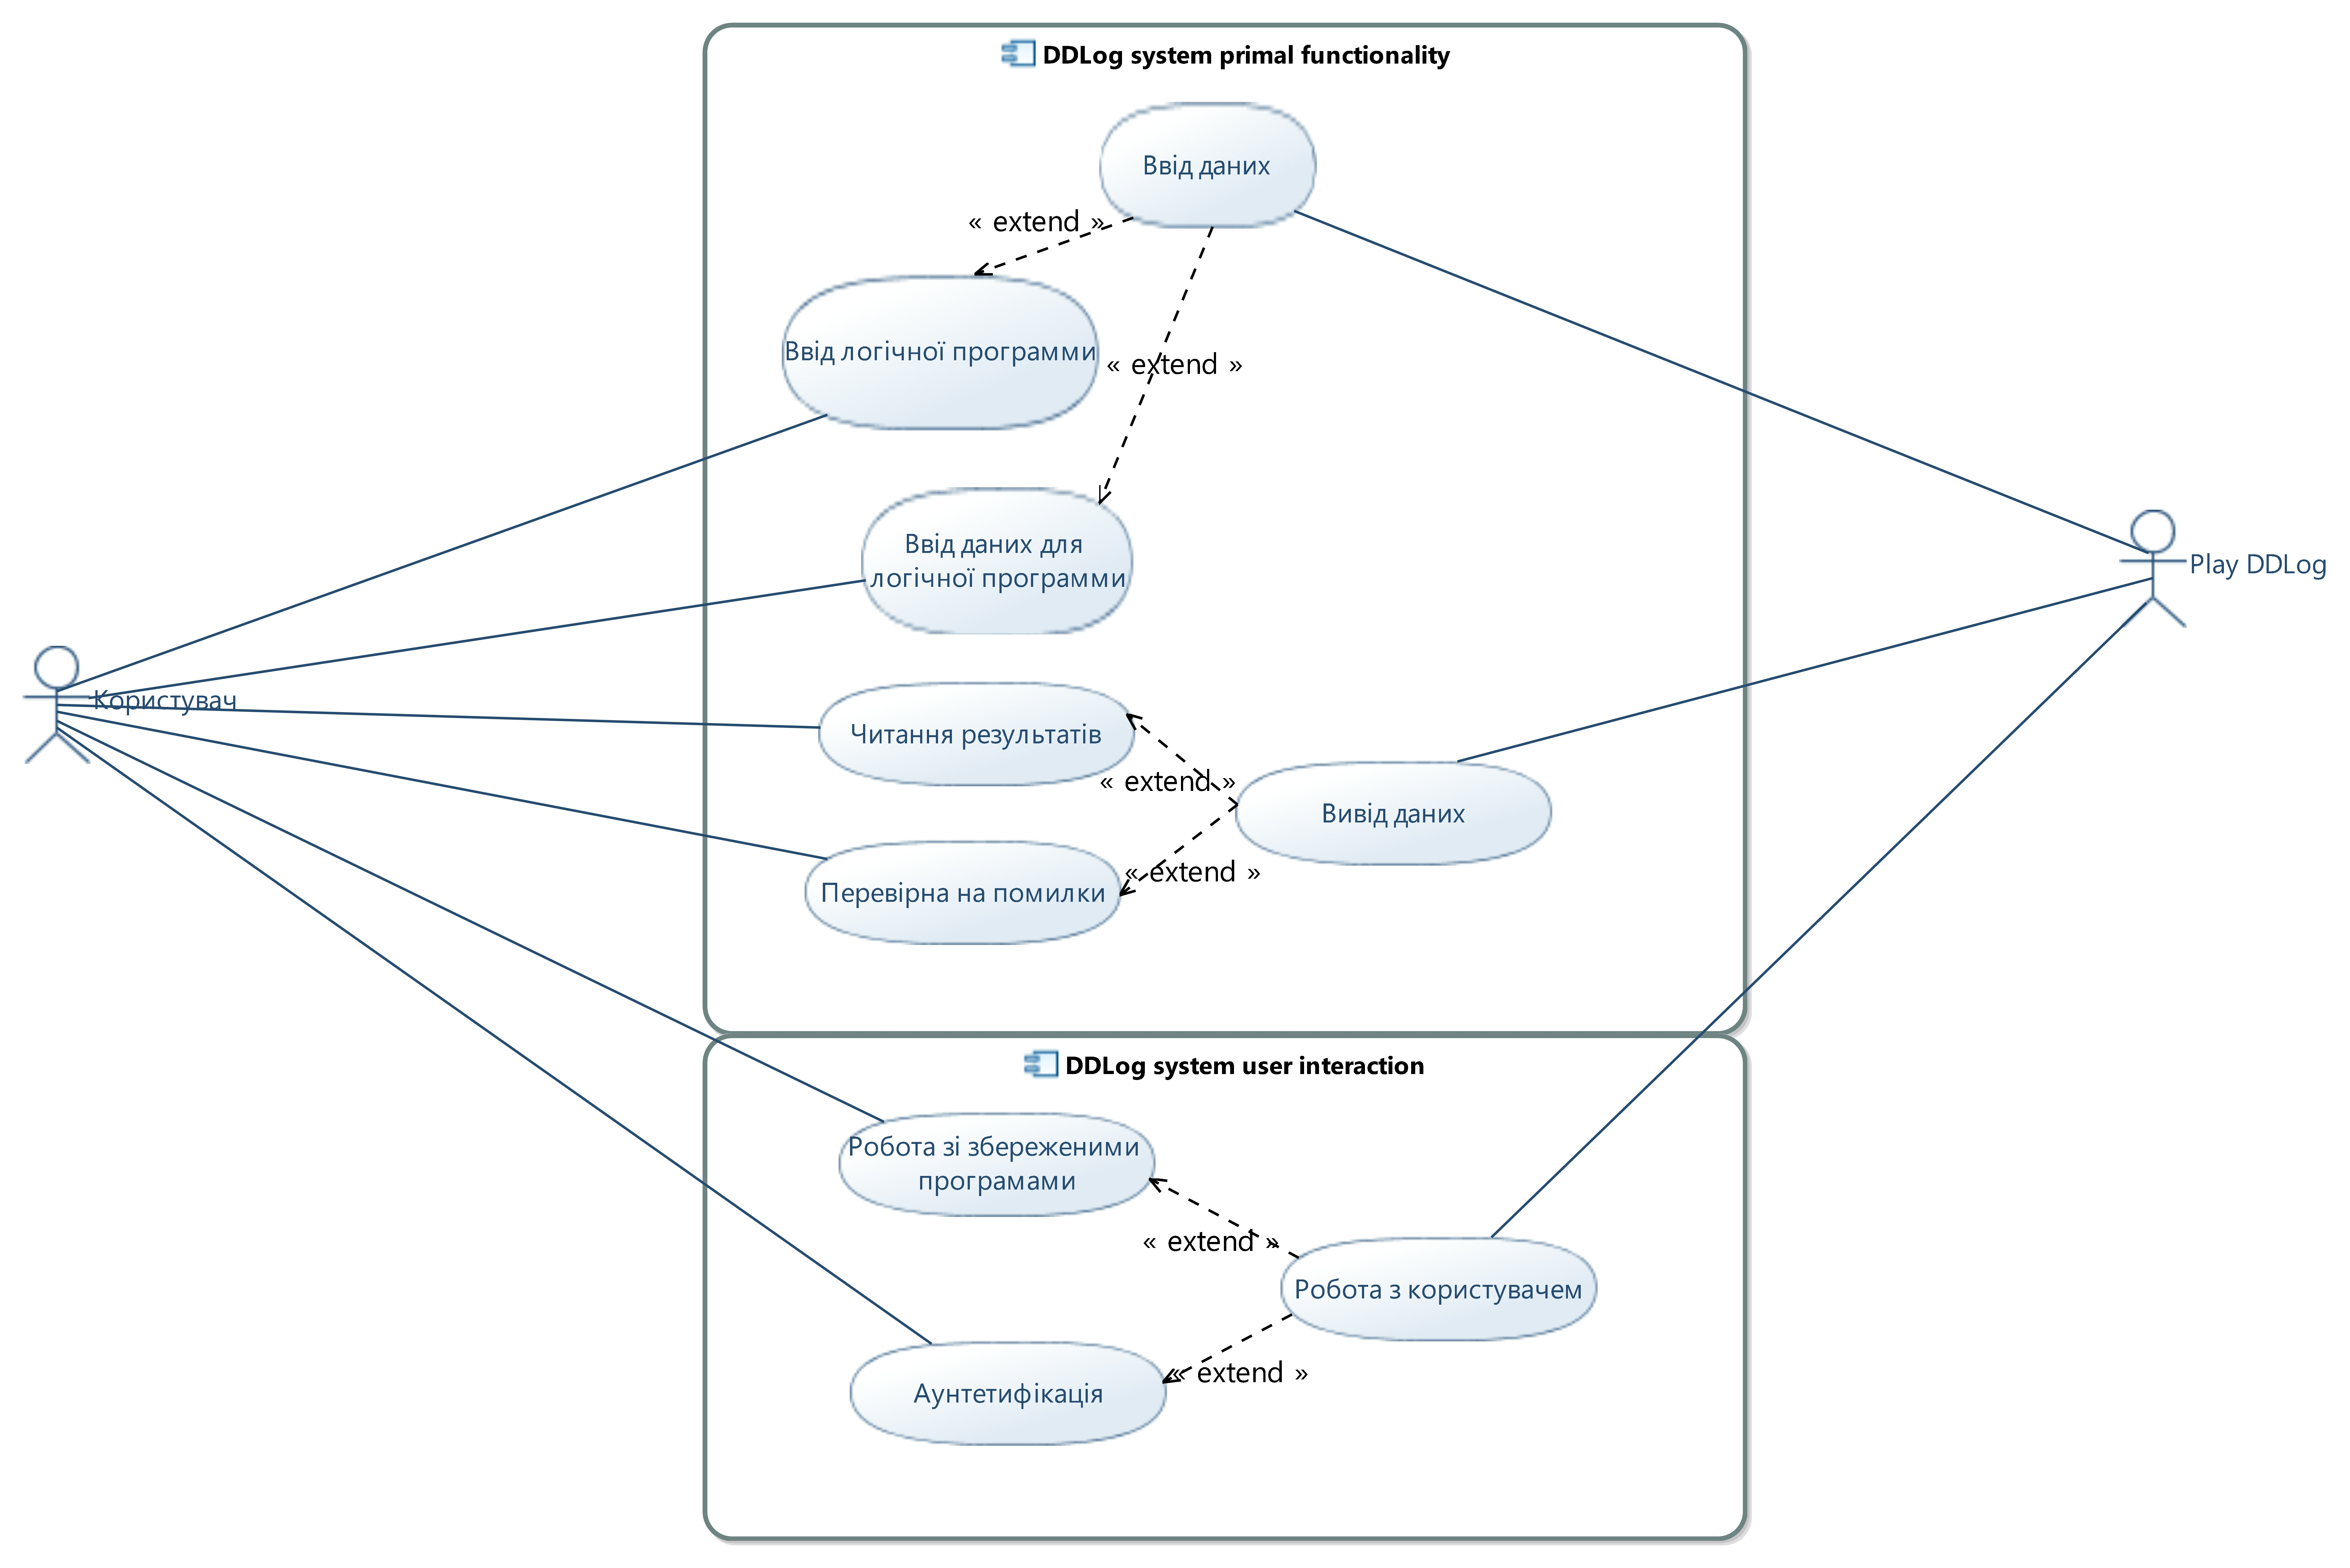
\includegraphics[width=12cm]{use_case_diagram}

Рисунок 2.1 - UML Use Case
\end{center}

\section{Характеристика задачі}

ІС призначенна для зручної роботи з логічними моделями мови DDLog. Це дозволяє досить швидко прототипувати моделі на цій мові. Персонал що працює з системою може використовувати її в будь-який час для тестування та використання програм DDLog.

Для зручності, система також повинна підтримувати роботу декількох користувачів, кожного з можливістю зберігати поточні моделі в ІС.
 
Інформаційна модель приведена нижче: 

\section{Вихідна інформація}

Вихідна інформація ІС: 

\begin{enumerate}
	\item Інтерактивна логічна модель
	\item Повідомлення про допущені в коді помилки, якщо ті були
	\item Результати взаємодії з логічною моделлю
\end{enumerate}

Деталі в таблиці відповідно номерам:

\begin{flushright}\small {Таблиця 2.1} \end{flushright}
\begin{center}
Вихідна інформація ІС
\small{
\begin{tabular}{ | c | c | c | c | c | }
\hline
 № з/п  & Ідентифікатор & Форма подання & Допустимий час затримки & Користувачі інформації \\ 
\hline
 1 & model & Елемент веб сторінки & 1-2 минути & Кінцевий користувач \\  
\hline
 2 & errors & Елемент веб сторінки & 1-2 минути & Кінцевий користувач \\  
\hline
 3 & results & Елемент веб сторінки & 1-2 минути & Кінцевий користувач \\  
\hline
\end{tabular}
}
\end{center}


\section{Вхідна інформація}

Вхідна інформація ІС: 

\begin{enumerate}
	\item Код логічної моделі.
	\item Будь-які вхідні дані цієї логічної моделі
	\item Запит на зберегання логічної моделі в ІС \ БД
	\item Запит на відтворення збереженної 
	\item Логін-пароль для ідентифікації користувача.
\end{enumerate}

Деталі в таблиці відповідно номерам:

\begin{flushright}\small {Таблиця 2.2} \end{flushright}
\begin{center}
Вхідна інформація ІС
\small{
\begin{tabular}{ | c | c | c | c |  }
\hline
 № з/п  & Ідентифікатор & Форма подання & Джерело \\ 
\hline
 1 & source & Елемент веб сторінки & Кінцевий користувач \\  
\hline
 2 & input & Елемент веб сторінки & Кінцевий користувач \\  
\hline
 3 & save & Елемент веб сторінки & Кінцевий користувач \\  
\hline
 4 & load & Діалог на веб сторінці & Кінцевий користувач \\  
\hline
 5 & login & Веб сторінка & Відвідувач веб сторінки \\  
\hline
\end{tabular}
}
\end{center}


\section{Математичне забезпечення та алгоритм функціонування системи}

Робота з мовою програмування DDLog передбачає обробку її коду. Це включає в себе:

\begin{itemize}
	\item Токенізація
	\item Побудова абстрактного синтаксичного дерева
	\item Передобробка AST
	\item Побудова словника правил, створення БД фактів.
\end{itemize}

Перші три єтапи можуть завершитися помилками, які будуть виведені користувачеві.

В результаті обробки коду, ми отримуємо опис логічної моделі. Цей опис надалі використовується ІС для інтерактивної роботи з нею.

Нижче наведено UML Sequence діаграмму, що ілюструє процесс роботи системи


\begin{center}

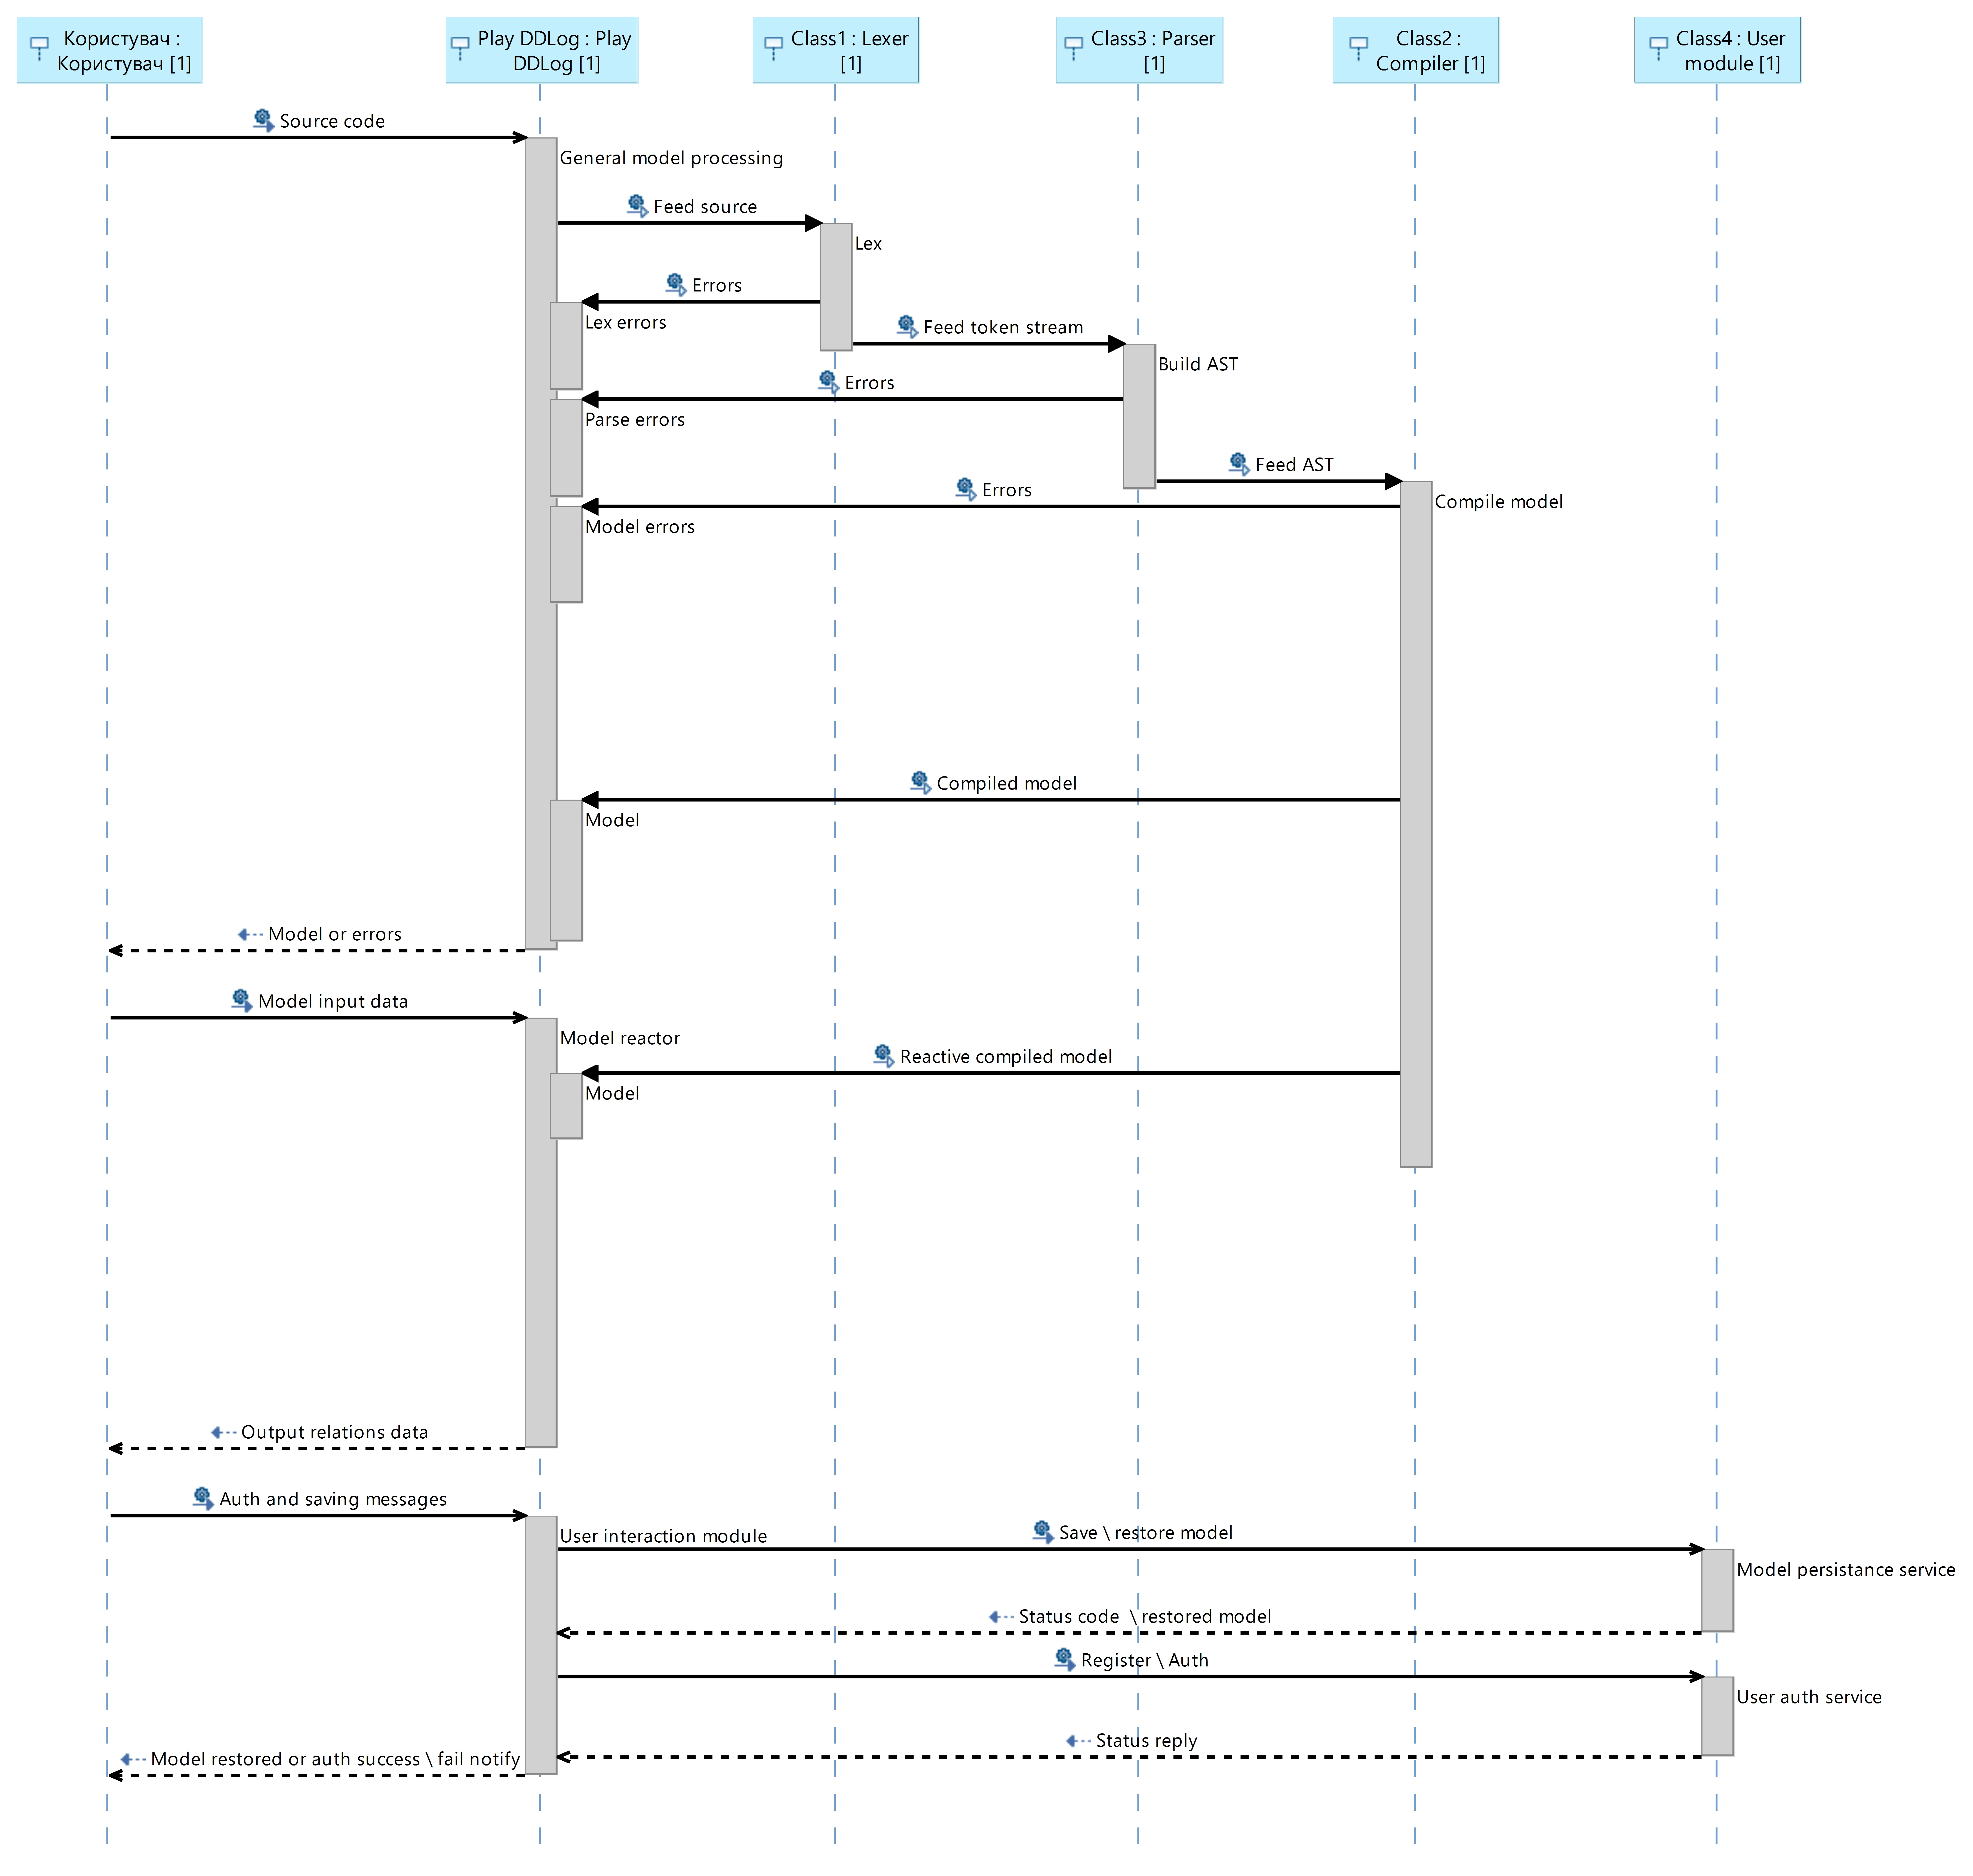
\includegraphics[width=12cm]{algorithm_sequence_diagram}

Рисунок 2.2 - UML Sequence
\end{center}

Зразок коду лексера надано в додатку А.


